\documentclass[tikz, border=10pt]{standalone}
\usepackage{pgfplots}
\usepackage{tikz}
\usepackage{amsmath}
\usetikzlibrary{patterns, intersections, fillbetween}

\begin{document}
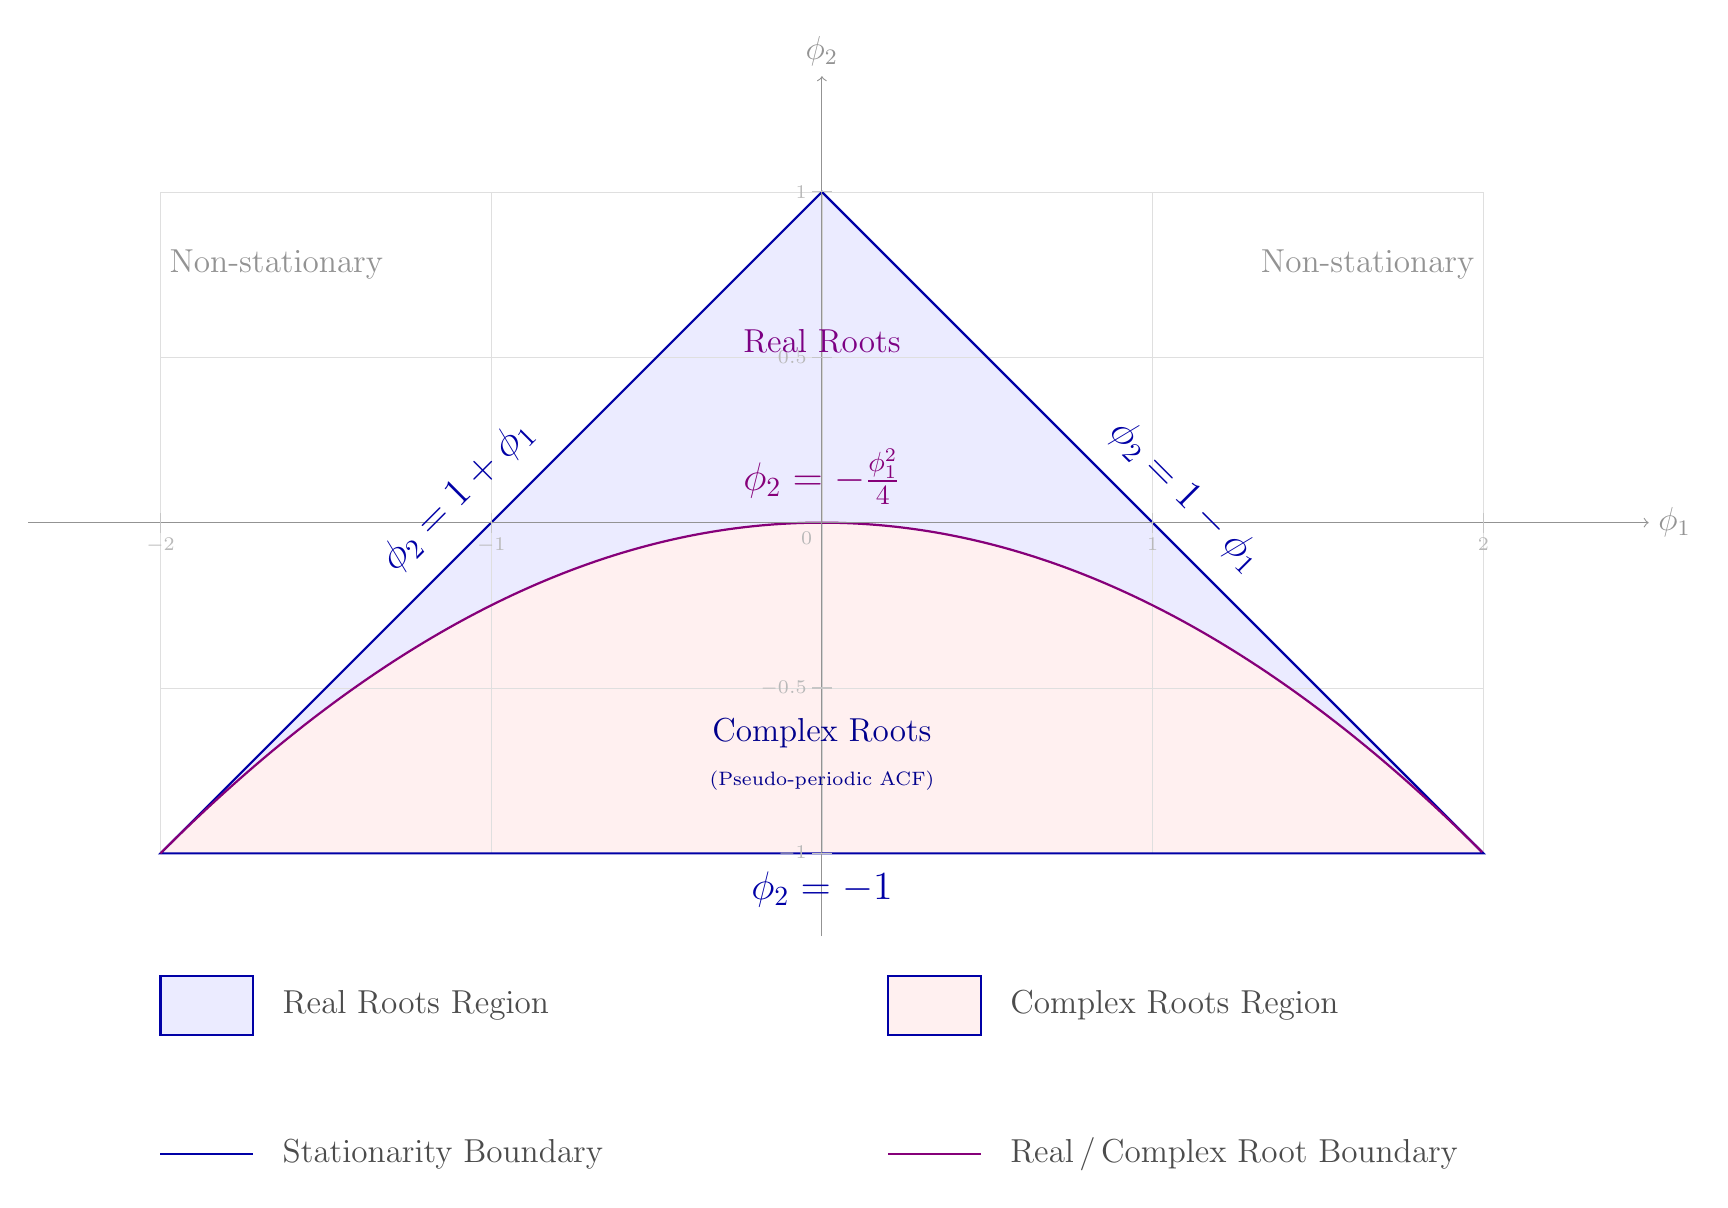
\begin{tikzpicture}[
  x=4.2cm, y=4.2cm,
  every node/.style={font=\small}
]

%% ── fill regions ─────────────────────────────────────────────────────────────

%% Complex-roots region: inside triangle AND above parabola phi2 = -phi1^2/4.
\fill[blue!8]
  (-2,-1)
  -- (0,1)
  -- (2,-1)
  -- plot[domain=2:-2, samples=200] (\x, {-\x*\x/4})
  -- cycle;

%% Real-roots region: inside triangle AND below parabola.
\fill[red!6]
  plot[domain=-2:2, samples=200] (\x, {-\x*\x/4})
  -- (2,-1)
  -- (-2,-1)
  -- cycle;

%% ── grid ─────────────────────────────────────────────────────────────────────
\draw[gray!25, very thin]
  \foreach \x in {-2,-1,1,2} { (\x,-1) -- (\x,1) }
  \foreach \y in {-1,-0.5,0.5,1} { (-2,\y) -- (2,\y) };
\draw[gray!35, very thin]
  (0,-1) -- (0,1)
  (-2,0) -- (2,0);

%% ── stationarity triangle ────────────────────────────────────────────────────
\draw[blue!65!black, thick] (-2,-1) -- (0,1) -- (2,-1) -- cycle;

%% ── parabola phi2 = -phi1^2/4 ────────────────────────────────────────────────
\draw[purple!70!blue, thick, domain=-2:2, samples=300, smooth]
  plot (\x, {-\x*\x/4});

%% ── axes ─────────────────────────────────────────────────────────────────────
\draw[->, gray!85, thin] (-2.4,0) -- (2.5,0)
  node[right, gray!85, font=\large] {$\phi_1$};
\draw[->, gray!85, thin] (0,-1.25) -- (0,1.35)
  node[above, gray!85, font=\large] {$\phi_2$};

%% ── tick marks and labels ────────────────────────────────────────────────────
\foreach \x in {-2,-1,1,2} {
  \draw[gray!45, thin] (\x,-0.03) -- (\x,0.03);
  \node[below, gray!55, font=\scriptsize, yshift=-2pt] at (\x,0) {$\x$};
}
\node[below left, gray!55, font=\scriptsize] at (0,0) {$0$};

\foreach \y/\lbl in {-1/{-1}, -0.5/{-0.5}, 0.5/{0.5}, 1/{1}} {
  \draw[gray!45, thin] (-0.03,\y) -- (0.03,\y);
  \node[left, gray!55, font=\scriptsize, xshift=-2pt] at (0,\y) {$\lbl$};
}

%% ── triangle edge labels ─────────────────────────────────────────────────────
\node[rotate=45, blue!65!black, font=\Large] at (-1.10, 0.08)
  {$\phi_2 = 1 + \phi_1$};
\node[rotate=-45, blue!65!black, font=\Large] at (1.10, 0.08)
  {$\phi_2 = 1 - \phi_1$};
\node[below, blue!65!black, font=\Large, yshift=-3pt] at (0,-1)
  {$\phi_2 = -1$};

%% ── parabola label: just above parabola apex at (0,0) ────────────────────────
\node[above, purple!70!blue, font=\Large, yshift=3pt] at (0, 0)
  {$\phi_2 = -\frac{\phi_1^2}{4}$};

%% ── region labels ────────────────────────────────────────────────────────────
\node[purple!65!blue, font=\large, align=center] at (0, 0.55) {Real Roots};

\node[blue!55!black, font=\large, align=center] at (0, -0.70)  {Complex Roots\\[2pt]\scriptsize(Pseudo-periodic ACF)};
%\node[blue!55!black, font=\small] at ( 1.28, -0.70) {Real roots};

\node[gray!85, font=\large] at (-1.65, 0.78) {Non-stationary};
\node[gray!85, font=\large] at ( 1.65, 0.78) {Non-stationary};

%% ── legend (positioned below the plot) ──────────────────────────────────────
\begin{scope}[shift={(-2.0, -1.55)}]
  % row 1
  \fill[blue!8]  (0,0)   rectangle (0.28, 0.18);
  \draw[blue!65!black, thick] (0,0) rectangle (0.28, 0.18);
  \node[right, font=\large, gray!60!black] at (0.34, 0.09)
    {Real Roots Region};

  \fill[red!6]   (2.2,0) rectangle (2.48, 0.18);
  \draw[blue!65!black, thick] (2.2,0) rectangle (2.48, 0.18);
  \node[right, font=\large, gray!60!black] at (2.54, 0.09)
    {Complex Roots Region};

  % row 2
  \draw[blue!65!black, thick] (0,-0.36) -- (0.28,-0.36);
  \node[right, font=\large, gray!60!black] at (0.34,-0.36)
    {Stationarity Boundary};

  \draw[purple!70!blue, thick] (2.2,-0.36) -- (2.48,-0.36);
  \node[right, font=\large, gray!60!black] at (2.54,-0.36)
    {Real\,/\,Complex Root Boundary};
\end{scope}

\end{tikzpicture}
\end{document}
